\documentclass[runningheads,a4paper]{llncs}
%\documentclass[a4paper,11pt]{report}
\usepackage{color,graphicx,url,wrapfig,glossaries,appendix,epigraph}
\graphicspath{{./images/}}
%\usepackage[dvips, bookmarks=true, unicode=true, breaklinks=true, pdftitle={Environment execution service}, pdfauthor={Aram Verstegen}, pdfsubject={Technical Computer Science - Bachelor's thesis}, pdfkeywords={NFC, mobile phones}]{hyperref}
%\makenomenclature
\makeglossaries
\begin{document}
\newcommand{\mytitle}{Security of NFC-enabled mobile devices}
\newcommand{\myauthor}{Aram Verstegen \& Mark Vijfvinkel}
\newcommand{\mycourse}{Research \& Development - Research 1, 2010-2011}
\pagenumbering{Roman}
\author{\myauthor}
\title{\mytitle}
\institute{Radboud University Nijmegen \\ \mycourse}
\maketitle
%\keywords{NFC, Secure Element, security}

\begin{flushleft}
\emph{Title:} \hfill  \mytitle \\
\emph{Authors:} \hfill \myauthor \\
\emph{Date:} \hfill \today \\
\emph{Course:} \hfill \mycourse \\
%\emph{Problem:} \hfill \\
\end{flushleft}

\begin{abstract}
New developments in mobile networking technology, which are intended to be used for payment and access control, deserve the attention of security researchers.
This paper aims to serve as both a general and a security-related introduction to mobile-phone based Near Field Communication systems.
\end{abstract}



%\newpage

%\tableofcontents
%\newpage

%\listoffigures
%\listoftables
%\printnomenclature
%\cleardoublepage

\setcounter{page}{1}
\pagenumbering{arabic}

\chapter{Introduction}
\newglossaryentry{PKI}{name={Public Key Infrastructure},description={A cryptographic methode for encrypting messages over untrusted networks.}}
\glsadd{PKI}

%\section*{Purpose}

%TODO Twee keer mobile device e.g. smartphone. 1x introduceren daarna placeholder gebruiken
\section{Near Field Communication} %(beetje dubbel)
Near Field Communication (NFC) is an upcoming wireless communication technology which will allow for new applications on mobile devices, e.g. smartphones.
It will allow a mobile device to communicate wirelessly over a short distance with other NFC-capable devices such as another smartphone, a payment terminal, a so-called 'smart poster' or an access control terminal.
There are two major use cases that sparked its development, namely mobile payments and access control. %MARK we zouden access control toch niet meer gebruiken?
For users of a mobile device NFC will increase the ease of use, because the user will be able to use a mobile device for paying (e.g. at a shop or candy machine) and use the same device to pay for public transport.
Theoretically the user doesn't have to carry a wallet anymore, only the mobile device.
For example, instead of using coins to pay for candy, you'll just wave your smartphone in front of the machine, you'll pay for the candy and the money will be taken out of your bank account. 

%plaatje van een NFC betaling

%TODO Telco's en gebruikers er bij
%TODO Manufacturers of what? - telefoons, NFC tags, ???
%\section{Stakeholders} % was dit niet overbodig om te noemen? MARK: volgens mij zei erik of alles noemen of eruit?
%NFC will be exploited by different stakeholders of the NFC Forum, which was started in 2004 to advance NFC technology.
%Stakeholders are hardware component manufacturers, mobile device assembling companies, SIM card producers, application developers and financial service institutions.
%And of course, let's not forget the user.
%Currently the Forum has 140 members, who all work together to promote the use of NFC. 
%Recently a few pilots have started in the Netherlands which allow users to pay with their mobile device and gain access.
%(misschien hier het voorbeeld noemen van OV chipkaart op de telefoon van Erik Poll).

\section{Applications}
While NFC is an emerging technology, there are some obvious areas in which it is likely to be applied. There are different parties throughout these areas, that are willing to exploit NFC technology. Some of these parties (hardware component manufacturers, mobile device assembling companies, SIM card producers, application developers and financial service institutions) are part of the NFC Forum, which was started in 2004 to advance NFC technology. Also users should be considered a major party in NFC technology.
For illustrative purposes a few applications in which NFC can be used are mentioned below.

\subsection{Payment}
Japanese telecommunications provider \textit{NTT DoCoMo} has initiated wide deployment of NFC technology in Japan, where virtually every issuer of payment cards supports the \textit{Sony}'s \textit{Felica Mobile Wallet} \cite{3g_japan}.
In this de-facto standard for mobile payment the mobile device emulates the behaviour of an RFID card, but in the future much more is possible by making use of the active communication possibilities of NFC. % TODO much more, zoals? MARK: Geen bron voor felica? Of waar komt dit vandaan?

% Referenties voor maken
In \cite{1555846} the authors investigate the security and usability, and as a whole the feasibility of NFC technology as a replacement for cash.
The authors concluded that their system is "highly usable and is even faster than cash under various common scenarios".

%In "Offline payments with Electronic Vouchers", the authors investigate the technical challenges of a system using cryptographically secure vouchers which can be exchanged between beneficiaries.
%They concluded the biggest limitation....
%MARK het bovenstaande werd weggelaten of wat was hier ook de bedoeling weer van?

\subsection{Public Transport}
Another application for NFC is public transport.
This way it is possible to use a mobile device to pay and gain access to i.e. a train, bus, or metro.
The Dutch infrastructure provider \textit{Trans Link Systems} (TLS), which was created as a joint venture between Dutch public transport companies to realise an electronic payment system for their services, have been investigating the feasibility of mobile phone-based payment applications using NFC. %referentie naar TLS
By holding your mobile device in front of a terminal you'll pay for a ticket or show your credit and a gate will open allowing you to enter.
The public transport system in the Netherlands uses this principle, it hasn't been implemented on a mobile device yet, but plans are being made. A mobile device has some advantages above a card, i.e. you can check the balance on your mobile device and increase it immediately. %MARK niet zo lekker stukje kan een bron bij, maar wat voor IEEE, ACM, scholar? Nog geen pilot in nederland :(

\subsection{Other applications}

Smart posters can be used to let a user interact with some piece of advertising.
For example it allows to transfer a URL or contact card to the receiving device.

Another application for NFC is in the healthcare system.
In \cite{RFIDHB} an application of NFC is used to measure the pressure in the eye.
A look at Google Scholar gave us the impression that the use of NFC in the healthcare system, is still in the development stage.
Therefore we will leave this application out of our research and recommend it for future work. %Mark niet zo sterk bewijs

\subsection{Implementation}
As mentioned above, there are different NFC applications (of which payment and public transport are the most important) and these applications are starting to be implemented. There are several reasons why NFC hasn't been implemented yet. First of all, the mobile devices that use NFC, still have to be made available to the consumer, but the consumer will only be interested if he or she can actually do something with NFC. So applications are needed, but therefore different parties have to work together. If i.e. a SIM-card is used as a secure element (see Chapter 3), a bank will need to trust the telecom provider and vice versa, but a bank doesn't like to use a, in their eyes, unsafe SIM-card and a telecom provider doesn't want someone else to mess with their SIM-card. Also the costs involved with trying to get all the shops using NFC, are quite large, because new payterminals have to be purchased.
So all parties have to participate and create agreements to get NFC off the ground, which is what they have been doing, only this takes time. %niet zo sterke zin en gebaseerd op de meeting met erik










\section{Security research}
While consumers might see these applications as a gadget that will make their lives easier, this development towards contactless payment systems rightfully raises questions from a security perspective.
Because NFC will be used in payment and access control, it should be assumed that attackers will try to exploit this technology for their own gain. 
Research has been done on the security of NFC in several areas, among which:

% TODO Referenties toevoegen
\begin{itemize}
\item Creating secure off-line payment applications
\item Trusted computing using mobile applications which are managed remotely
\item Network attacks against \textit{Wireless Personal Area} (WPAN) \textit{Networks} (e.g \textit{Denial of Service}, \textit{Snooping}, \textit{Man-in-the-middle}, etc.) \footnote{Even though NFC isn't strictly a WPAN system as it only allows for 2 communicating parties, this paper also covers network attacks against NFC.} %WPAN afkorting introduceren
\item Intrusion detection mechanisms for WPANs
\item Mitigations agains privacy issues related to wireless payment systems
\end{itemize}

To our knowledge there has been no succinct, definitive overview leading from the system organisation to the security architecture and the known vulnerabilities of NFC systems.
% "Did you google scholar around for this?"
What we hope to accomplish with this paper is to provide the reader with an introduction to NFC security-related research currently ongoing.
%In addition to this we hope to be able to identify specific applications in which we foresee vulnerabilities.
% "Introduction to NFC security _research_"
% vs "Introduction to NFC security _issues/architecture_"
% Naar welk aspect kijken wij? - Verderop in 1.5 geven jullie hier beter antwoord op

\newpage

\section{Overview}
In chapter \ref{chap:applications} we will briefly summarize some of the applications NFC will likely be used for.
In chapter \ref{chap:hardware_architecture} we will present an overview of the hardware, software and communication architecture of a NFC-enabled mobile device.
%\section{...}
%Further we will look into the possibilities that NFC offers.
In chapter \ref{chap:known_vulnerabilities} we will summarize security issues on vulnerabilities in NFC or NFC-like applications.

Based on the architecture and these vulnerabilities, we present a number of foreseen vulnerabilities and explain some possible countermeasures against these foreseen vulnerabilities in chapter \ref{chap:foreseen_vulnerabilities}.


%Bronnen:
%IEEE artikelen:
%Near Field Communication Network Services
%Vulnerability Analysis and Attacks on NFC-enabled Mobile Phones

\section{Applications}
While NFC is an emerging technology, there are some areas in which it is likely to be applied.
Various parties throughout the areas of public transport, building security and payment card companies have expressed interest in employing NFC technology.

For illustrative purposes a few applications in which NFC can be used are mentioned below.

\subsection{Public Transport}
%Another application for NFC is public transport.
%This way it is possible to use a mobile device to pay and gain access to i.e. a train, bus, or metro.
%By holding your mobile device in front of a terminal you'll pay for a ticket or show your credit and a gate will open allowing you to enter.
Public transport companies in the Netherlands have largely adopted RFID technology for payment and access control, through infrastructure provider \textit{Trans Link Systems} (TLS).
%TODO referentie naar pilot - DONE?
TLS was created as a joint venture between Dutch public transport companies to realise an electronic payment system for their services. They have also been investigating the feasibility of mobile phone-based payment applications using NFC.
The use of NFC technology for payment in public transport is currently considered unfeasible by TLS because it would require users to own an NFC-enabled handset; devices which so far have no significant market penetration in the Netherlands.
Also, the relatively high cost of an NFC-enabled phone as well as the requirement to keep the device powered on during the length of a trip are aspects of NFC which go against TLS's aim for a low threshold in using their electronic ticket system.
%It would also prohibitively expensive for most users and NFC phones are not widely available.
TLS are still investigating the future possibilities of adopting NFC technology as an alternative payment method. \cite{OVchipkaart} %referentie naar TLS
%hasn't been implemented on a mobile device yet, but plans are being made.
A mobile device has advantages over a card, e.g. you can check the balance on your mobile device and increase it immediately by paying online. Therefore, the user doesn't have to go to a terminal, which will increase the user experience.
Support for NFC-enabled devices in TLS's system could improve user experience by giving users the option to check or increase the balance of their electronic ticket account at any given time, alleviating the oft-heard complaint of currently only being able to do so at (most) train stations.


%MARK niet zo lekker stukje kan een bron bij, maar wat voor IEEE, ACM, scholar? Nog geen pilot in nederland :(


\subsection{Payment}
Japanese telecommunications provider \textit{NTT DoCoMo} has initiated wide deployment of NFC technology in Japan, where virtually every issuer of payment cards supports the \textit{Sony}'s \textit{Felica Mobile Wallet} \cite{yamauchi2006intensive}.
In this de-facto standard for mobile payment the mobile device emulates the behaviour of an RFID card, but in the future much more is possible by making use of the active communication possibilities of NFC. For example, by being able to transfer money between two people, NFC technology might become a replacement for cash. E.g. the payment application \textit{mFerio} should be as easy to use and be as available as cash. It should also improve accuracy and speed, while still meeting security criteria like transaction integrity, anonymity, tamper-resistance, impossibility to replicate and theft resilience. 
\textit{mFerio} uses NFC, because of three advantages above other mechanisms, namely it has a short range (harder to intercept transactions), it is quick and easy to set up and a user knows with which device communication is set up. The secure element (SE) in \textit{mFerio} contains cash and personal details of the user, which will not be accessible by criminals if the secure element is hardware protected \cite{1555846}.

A possibility to create an offline payment system, is the use of electronic vouchers. A user can recieve an 'eVoucher' by an SMS from an issuer and transfer the eVoucher to other users (by NFC, SMS or a RFID tag) and payment terminals. Users are also able to check the balance, history and expiration date of the eVouchers. 
There are three risks concerning this implementation, first the possibility of copying the eVouchers, second counterfeiting them and third loss of eVouchers in a transaction. The secure element will only accept software from a Trusted Service Manager, which will have a private key for authentication to the SE. The SE will store the eVouchers and also encrypt them, if a user decides to sent them to another user. \cite{1592613}

%In \cite{1592613} the authors investigate the technical challenges of a system using cryptographically secure vouchers %which can be exchanged between beneficiaries.
%\textbf{TODO} add their conclusion.
% TODO conclusion
%They concluded the biggest limitation....
%MARK het bovenstaande werd weggelaten of wat was hier ook de bedoeling weer van?

\subsection{Advertisement}
Advertisement is another area in which NFC can be used. By equipping advertisements (e.g. billboards, flyers, posters) with a NFC/RFID-tag, users can check the details of a product immediately on their mobile phone. Or by supplying the tag with an URL, a user can immediately visit a website and take further action there, e.g. sign-up or fill in a form. As we will see in chapter 4, this can create a security problem for a user that is unaware. \cite{10.1109/ARES.2009.46}

\subsection{Access Control}
It is also possible to use NFC to gain access to a certain area e.g. a building or room. The company Nedap Healthcare developed an application for caretakers in the home care business. By using an NFC enabled phone, the caretaker can gain access to the house of the client. Upon arrival and leaving the caretaker holds the phone next to the membershipcard of the client, which will register the visit of the caretaker and given care. \cite{Nedap1}, \cite{Nedap2}

%\subsection{Healthcare}
%Another application for NFC is in the healthcare system.
%In \cite{RFIDHB} an application of NFC is used to measure the pressure in the eye.
%A look at Google Scholar gave us the impression that the use of NFC in the healthcare system, is still in the development stage. %ERIK: niet zo sterk, vervangen door "The current scientific literature gives the impression...", Sommige van deze publicaties noemen.
%Therefore we will leave this application out of our research and recommend it for future work. %Mark niet zo sterk bewijs


%\section{Implementation} %goede titel nodig?
%As mentioned above, there are different NFC applications (of which payment and public transport are the most important) and these applications are starting to be implemented. There are several reasons why NFC hasn't been implemented yet. First of all, the mobile devices that use NFC, still have to be made available to the consumer, but the consumer will only be interested if he or she can actually do something with NFC. So applications are needed, but therefore different parties have to work together. If i.e. a SIM-card is used as a secure element (see Chapter 3), a bank will need to trust the telecom provider and vice versa, but a bank doesn't like to use a, in their eyes, unsafe SIM-card and a telecom provider doesn't want someone else to mess with their SIM-card. Also the costs involved with trying to get all the shops using NFC, are quite large, because new payterminals have to be purchased.
%So all parties have to participate and create agreements to get NFC off the ground, which is what they have been doing, only this takes time. %niet zo sterke zin en gebaseerd op de meeting met erik


% Kip & ei probleem
% Genoeg NFC handsets <-> apps
% trust: telco <-> bank <-> telefoonmaker
% kosten voor payment -> nfc reader bij alle kassa's
% iedereen moet mee doen

% MARK weet niet zo goed wat ik met het onderstaande commentaar moet doen

% SIM - 4k ram 16k rom 64k eeprom

%            trust
% security <             afluister
%            aanvaller < relay attacks
%                        malware

%\section{Pilot programs}
% /* promising secure element alternatives for NFC technology.
%TODO door wie, hoeveel participanten etc is wel nuttig om te weten
%TODO Er wordt er ook maar 1 genoemd

%In London there has been a pilot between November 2007 and May 2008, during which 78 percent participants were interested in using this technique.
%According to networking hardware vendor \textit{Juniper Networks}, 700 million of NFC-enabled mobile phones will be in use by 2013. 
%One of the factors holding back the widespread adoption of NFC, is stakeholders (e.g. banks, mobile providers and public transport companies) have so far been unable to agree on standardization of the required security implements. 

% sorry maar even herschreven om niet meteen heel specifiek te gaan.
%The secure element consists of hardware, software, interfaces and protocols in a mobile device.
%It provides a secure area for storage, running of applications, protection of payments and can be used for authentication  and for applications which need security mechanism.
% dit stukje is niet zo precies, en moet in de introductie minder technisch uitgelegd worden denk ik

%TODO dit moet eigenlijk ergens anders heen
%There are several reasons why NFC hasn't been implemented yet.
%First of all, the mobile devices that use NFC, still have to be made available to the consumer, but the consumer will only be interested if he or she can actually do something with NFC.
%So applications are needed, but therefore different parties have to work together.
%If i.e. a SIM-card is used as a secure element (see Chapter 3), a bank will need to trust the telecom provider and vice versa, but a bank doesn't like to use a, in their eyes, unsafe SIM-card and a telecom provider doesn't want someone else to mess with their SIM-card.
%Also the costs involved with trying to get all the shops using NFC, are quite large, because new payterminals have to be purchased.
%So all parties have to participate and create agreements to get NFC off the ground, which is what they have been doing, only this takes time. %niet zo sterke zin en gebaseerd op de meeting met erik


\section{System Architecture}
\label{chap:hardware_architecture}
With the development of mobile payment applications comes the requirement to ensure the security of the financial assets involved.
An architecture for the application of mobile devices for `electronic cash' must provide a means to authenticate transactions before authorizing their execution, whether that be on-line or off-line.

%In electronic payment applications there are at least three roles to be distinguished: consumers, merchants and payment providers.
%For each inter-party transaction, the parties must be identified and authenticated.
%The problem faced by system architects in developing secure payment applications is that a breach of security can occur within each of these parties' assets.

%Consumers and retailers both need to trust a payment provider (e.g. a bank) to process their payment transactions, and in return the payment provider must verify both parties are making rightful claims to their accounts.
%There are now three participants in the transaction instead of two, and - ruling out internal sabotage - two points of potential malice rather than just one.
%This creates a situation where the burden to authenticate a transaction is twice as great on the payment provider as it would be for either participant in a direct two-party transaction.
Traditional mechanisms of authenticating payment transactions in electronic banking rely on verification of the data stored on the magnetic stripe and verification of the client's signature on the card by visual inspection.
Transactions can be authenticated more securely by using a cryptographic solution relying on \textit{Integrated Circuit Cards}.

\textit{Integrated Circuit Cards} (ICCs), commonly known as smart cards or chip cards, are cards which contain an integrated circuit which can communicate to the outside world via contact points on the card.
The microchips embedded in these cards can be used to cryptographically sign data using a preconfigured secret key which is contained within the chip.
\cite{herzberg2003payments,khu2002using}
The chips in smart cards are designed to minimize the risk of an attacker extracting the secret key it holds.
Smart cards can be issued with various anti-tampering mechanisms, adding to the intrinsic tamper-resistance of the chip due to its small scale. \cite{kömmerling1999design}
Europay, Mastercard and Visa have jointly designed the EMV standard for smart card interoperability describing a secure means of transaction authentication using smart cards. %, which has been largely adopted by the banking industry and is in widespread use.
The enhanced security provided by the EMV system has effected a liability shift where the non-EMV compliant party can be held liable for any fraud committed. \cite{povey2008assessing}
%been adopted by  which has lead to the widespread deployment of smart cards.
%Smart cards used in EMV hold an encryption algorithm and secret key known only to the bank, which are used to sign transactions.
%Smart cards are called 'smart' because they contain an embedded microchip which is able to not only store data, but also run code.

%This 
%Transactions in the EMV system are authorized after establishing the card is authentic and verification of the cardholders identity.
%Establishing the authenticity of the card can be accomplished in two ways, to be decided upon by the ICC or the payment terminal.

%\begin{enumerate}
%\item \textbf{Static Data Authentication (SDA)

%\end{enumerate}
%A more secure means of verifying transactions would be a mechanism where the user would.
%The payment provider would share with the user containing two keys: one which is known only to the payment provider while in possession of the user, whereas the other key is publicly known.
%The user is also issued a \textit{Personal Identification Number} (PIN) which is a shared secret between the user and the card issuer.

%As an analogy, imagine the secret key functions as a padlock which the user can close, but not open.
%It may be in the user's possession, but extracting the combination from the lock would in most cases destroy it.
%Using this lock, the user can transmit the 'locked' shared secret to the payment provider, which on the receiving end can produce the same in order to authenticate his or her transaction.

%A payment provider
%TODO Leg uit hoe je met trust omgaat in electronisch bankieren
A similar application of smart cards can be found in mobile telephony networks.
Worldwide, most mobile telephones make use of the \textit{Global System for Mobile Communications} (GSM) system.
The GSM standard already provides a mechanism for authentication to the network by means of a smart card, albeit in a different form factor, called a \textit{Universal Integrated Circuit Card} (UICC).
In GSM networks, the UICC is running a \textit{Subscriber Identify Module} (SIM) application, which provides a mobile handset access to the encryption routines required for authentication on the network while the required secret key remains stored securely inside.

\begin{figure}
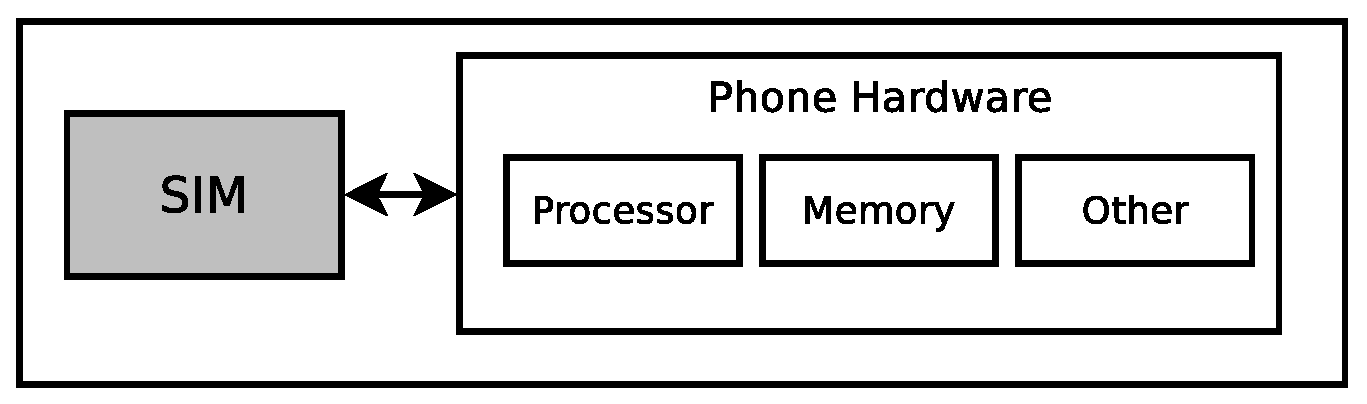
\includegraphics[width=0.9\textwidth]{images/SIM_in_GSM}
\caption[UICC running SIM application in GSM]
{
A UICC (SIM) card as used in GSM holds the Mobile Network Operator's secret key.
}
\label{fig:gsm_sim}
\end{figure}

These types of cards, also known as SIM cards, remain property of the \textit{Mobile Network Operator} (MNO) after distribution, much like a bank card or passport remain the property of their respective issuers. %TODO referentie
The contents of the card may normally not be modified by third parties.
Due to this, the current generation of mobile devices lacks a common infrastructure for third parties to make use of such a secure computation platform for their own applications.

%These third parties need to be elevated to the role of \textit{Trusted Service Manger}
%MARK: In de tekst hieronder moet duidelijk worden, dat NFC eist/vraagt dat een UICC wordt opgedeeld voor verschillende applicaties

% ERIK: SIM is een voorbeeld van een "Secure Element". Een Secure Element kan ook een andere smartcard chip in de telefoon zijn.

% In de telefoons die 'we' hebben is de SE geen onderdeel van de SIM, maar een los (al dan niet trusted) component.
%MARK: zullen we dit verder uitbreiden in het architectuur hoofdstuk en dit hier niet noemen?


%ERIK Waarom is de architectuur van GSM zoals-ie is & hoe breidt NFC dat uit? Er zijn tig opties van NFC telefoons, dus we kunnen niet overal diep op ingaan.

\subsection{Secure elements}
%Modern RFID cards can have features similar to smart cards, which means that NFC devices aiming to be truly compatible with RFID applications must also allow for similar functionality.
Just like SIM cards and RFID cards, NFC-enabled handsets require a secure storage and processing module to be included in their design as conventional storage on and operation of mobile devices are liable to tampering by the user or malicious third party.
%NFC, being grounded in RFID technology, provides some security capabilities previously unavailable in mobile devices.
%These capabilities require storage of sensitive data and code, for which a \textit{Secure element} is needed.
%Currently, four different configurations for a secure element are possible, of which the integration on a regular UICC/SIM is suggested as the most likely candidate to be used.
Secure storage for NFC applications similar to that provided by smart cards has been implemented in the \textit{Secure Element} (SE) architecture.
SEs can be updated over-the-air by a \textit{Trusted Services Manager} (TSM), provided the TSM's certificate is trusted by it.
Several possible configurations proposed by \textit{GlobalPlatform}, the industry forum for smart card infrastructure development, are outlined below. \cite{Reveilhac:2009:PSE:1548884.1549404,GlobalPlatformSEs}

%The secure element to be used is a \textit{Universal Integrated Circuit Card} (UICC).
%This is a smartcard which is used in a mobile phone to connect to the GSM and UTMS network. % UICC toevoegen aan glossary, Uitleggen dat het SIM is
%Making use of a UICC is preferred because it has been deployed in real applications where it has proven to be reliable.
%It is re-usable and standardized, which means a user can switch handsets easily, their personalized secure. 


%\textbf{TODO}
%A good reference on the feasibility of secure data and code in mobile devices is given in \cite{Reveilhac:2009:PSE:1548884.1549404}.
%Explain that the technical workings of these different devices are equivalent, but different configurations belong in different trust models.


%ERIK: figuren toevoegen van verschillende telefoon architecturen. 

% SIM ---> telefoon		SIM = secure, tamper-resitent, authenticatie van telefoon aan het netwerk	marketing redenen (onderscheid welke onderdelen van wie zijn) SIM is van de telco
% a SIM ---> telefoon ---> SE 	SmartMX contactless smartcard  (nokia)
% b SD kaart als a maar vervangbaar SE
% c NFC-SIM

%The problem of a malicious user can be mitigated by making use of a \textit{Secure Element} (SE) for storing sensitive information.
%Because of its sheer microscopic scale, it is very difficult and costly for an attacker to tamper with the function of this device.

%Below we will discuss a number of different ways such a secure element can be implemented on a mobile device. 

%\subsubsection{Integrated Secure Element}
\begin{enumerate}

\begin{item}
One option would be to integrate the SE in the handset hardware directly.
This works for the intended cryptographic use, but limits the device to communicate with the services using its pre-programmed certificates, unless it is capable of securely updating itself with new certificates.

%Nokia has released a phone like this in 2006 (the Nokia 6131 NFC) . %with NFC as a feature.
%The architecture of this phone consists of a SIM card, antenna and an internal Secure Element.
%The same layout of this architecture can also be used in other mobile devices, see figure \ref{fig:integrated_se}.

The handset hardware consists of the usual components like a processor, memory and possibly others, but also the hardware to provide NFC features and an embedded secure element.
The downside to this design is that the data contained in the SE is not easily portable to a new NFC device.
%The secure element stores sensitive data and enables tag and smart card emulation.
%In the case of the Nokia phone it is divided in two subcomponents, a Java Card, used for payment, and Mifare 4k, used for ticketing.

\begin{figure}
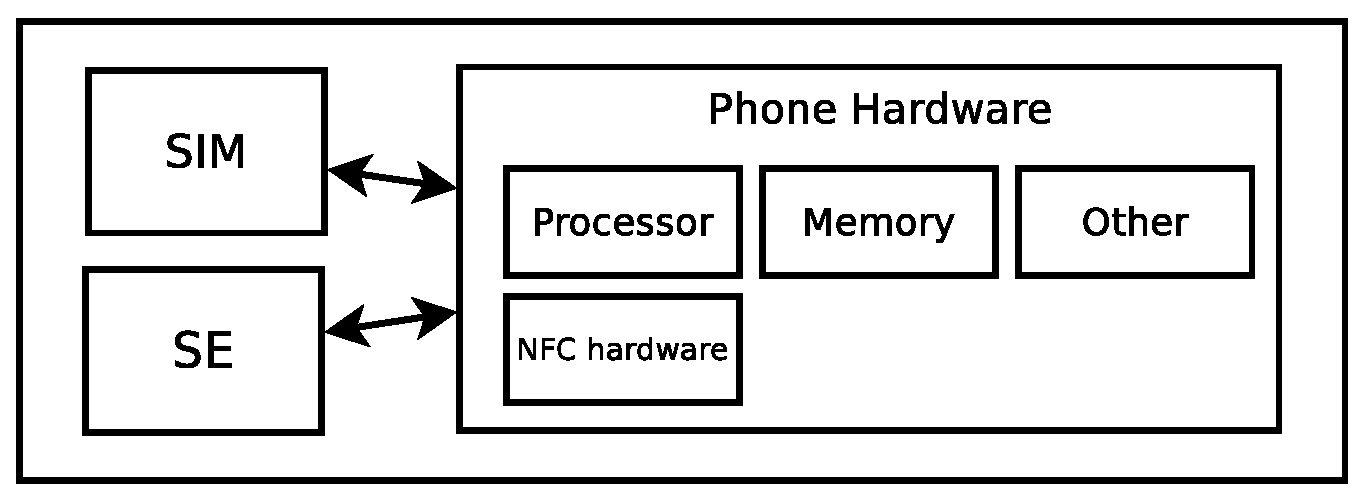
\includegraphics[width=0.9\textwidth]{images/phone_with_SE_nokia}
\caption[Handset with embedded Secure Element]
{
An embedded secure element
}
\label{fig:integrated_se}
\end{figure}
\end{item}

%security problems for this architecture:

%\subsubsection{Modular Secure Element}
\begin{item}
Another option is a flash memory card like a \textit{Secure Digital} (SD) card which houses all the hardware needed to enable NFC and also the secure element, as depicted in figure \ref{fig:modular_se}.
%( http://www.nearfieldcommunicationsworld.com/2009/01/12/3485/tyfone-puts-nfc-into-microsd-cards/)
In this configuration a third party can issue an SD card to its customers which provides NFC functionality without relying on any aspect of the handset to handle confidential data.
\begin{figure}
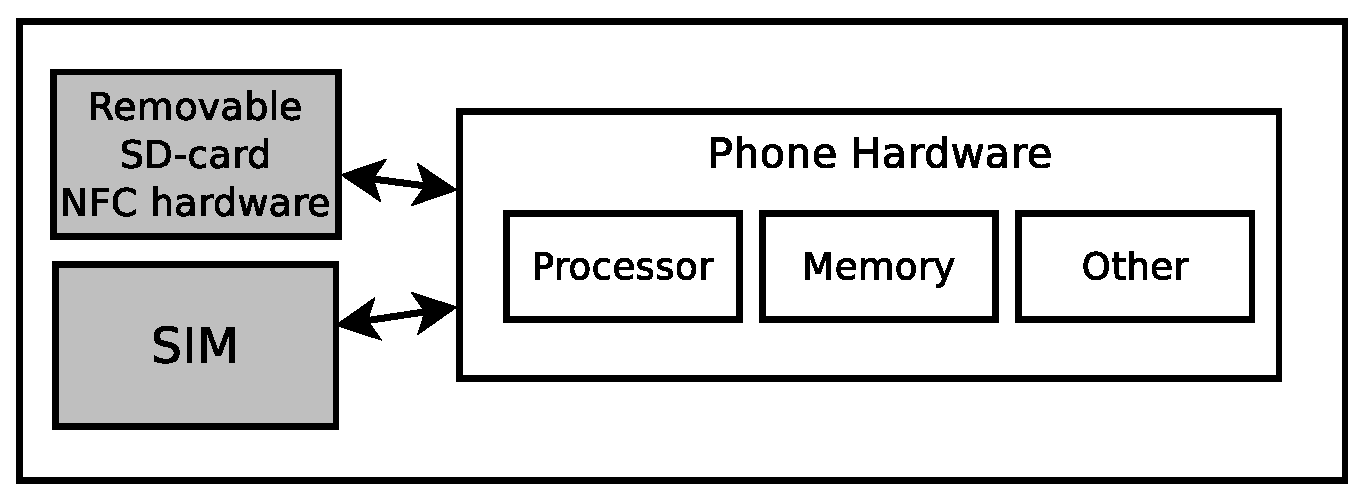
\includegraphics[width=0.9\textwidth]{images/SD_NFC}
\caption[SE in SD package]
{
A secure element in an SD package
}
\label{fig:modular_se}
\end{figure}
\end{item}

%security problems for this architecture: SD card might get stolen and used by somebody else.
%\subsubsection{Multiple SIM cards}
\begin{item}
Related to the above architecture is the one depicted in figure \ref{fig:multi_sim}.
Here the architecture consists of a handset with multiple UICC slots.
In this design various applications have access to their own UICC which takes on the role of an SE.
This way, applications from different providers can coexist on the handset, without the need for them to trust one another or a TSM operating on their behalf. % there is no problem with splitting the resources of one SIM card and the trust issue between different companies.
\begin{figure}
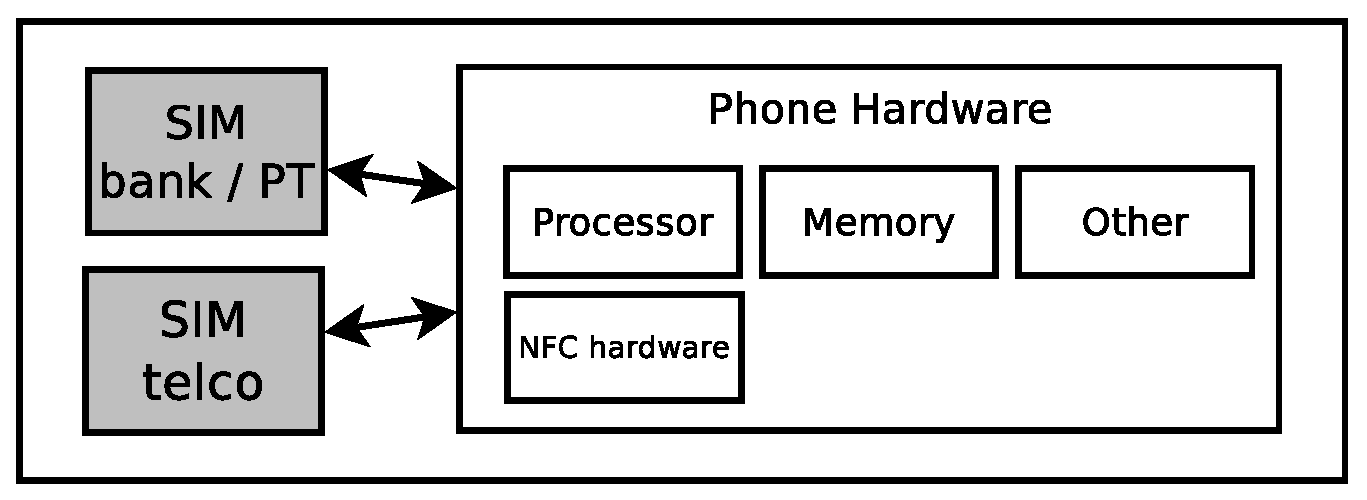
\includegraphics[width=0.9\textwidth]{images/meerdere_sims}
\caption[Multiple SIM cards]
{
Multiple SIM cards for different applications
}
\label{fig:multi_sim}
\end{figure}
\end{item}

\begin{item}
%\subsubsection{Trusted SIM card}
It is also possible to split the resources available on the SE between various parties, granted they trust each other to not abuse the privilege of being able to access one another's data.
This sharing of resources is possible because smart cards in general are becoming more powerful.
This makes two different architectures possible.
The first one, as pictured in figure \ref{fig:sim_se}, uses the SIM card as secure element.
In this design, the handset will include the NFC communication hardware and utilize a UICC (SIM card) with applications from the Mobile Network Operator and applications from various third parties chosen by the user, e.g. a bank for payment and a public transport company. 
The second option resembles a combination of the first one and the one with the SD card architecture.
Here a SIM card has all the hardware needed to make NFC possible and it also acts as a secure element (see figure \ref{fig:integrated_se}).
Like the first option, the resources of the SIM card will be split among the involved parties.
\begin{figure}
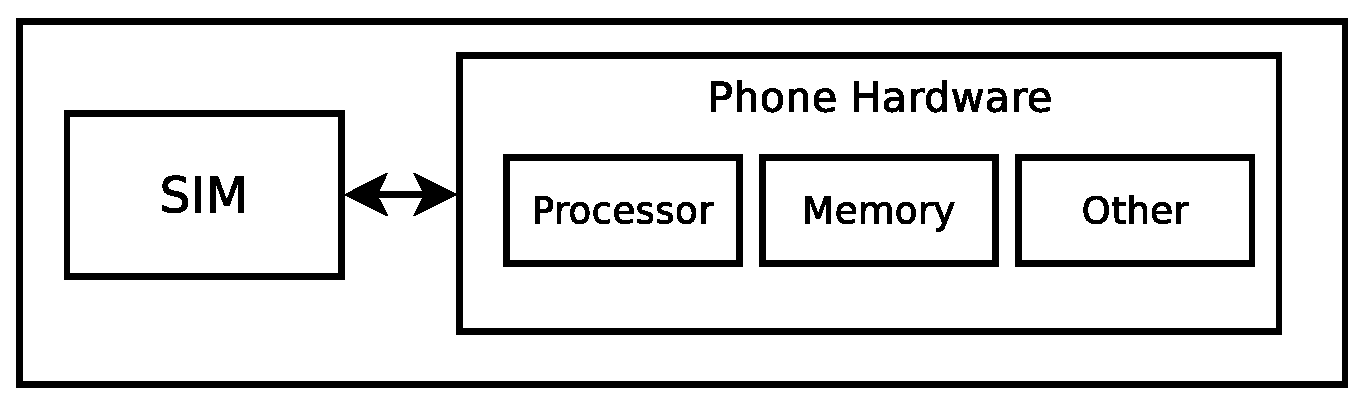
\includegraphics[width=0.9\textwidth]{images/SIM_is_SE}
\caption[Trusted SIM cards]
{
Trusted SIM card running multiple applications
}
\label{fig:sim_se}
\end{figure}
\end{item}

\end{enumerate}

%hier moet nog een bron voor gevonden worden
%security problems for this architecture: SIM card might get stolen and used by somebody else
%hier moet nog een bron voor gevonden worden
%security problems for this architecture: SIM card might get stolen and used by somebody else


%\textbf{TODO} A good reference for cyclic dependency of stakeholders can be found in the GlobalPlatform technical report.


% TODO hoort bij Wireless communication, terwijl 3.2 (Secure Elements) heel ergens anders over gaat
%\subsection{Standardization}
%NFC has been described by NFCIP-1 (Near Field Communication Interface Protocol 1) first on ISO18092, ECMA340 and ETSI %TS102 and also NFCIP-2 defined in ISO 21481, ECMA352 and ETSI TS102 312.
%With NFCIP-2, NFC became compliant with the RFID standards of ISO14443 and ISO15693.


% diagram van NFC communicatie

%TODO RFiD card vs NFC - verschil vd terminal
%                      - live GSM verbinding met de bank
%TODO Online vs Offline
%                      - privacy gevoeligheid

%\section{Wireless communication}
%The distance at which the NFC communication takes place is 10 cm, operates at the 13.56 MHz frequency and it has a transfer speed of 106, 216, 424 kbit/s.
%promising secure element alternatives for NFC technology. */


%\subsection{Advantages and Limitations}
%\textbf{TODO}

% Toetsenbord en display feature (semi-trusted terminal, moeilijker te tamperen)

% Voorbeeld telefoon met gewone sim en NFC SD card adapter
% Bankier kan heir apps op installeren

% Voorbeeld telefoon met meerdere sims

% Vorobeeld SIM en losse SE, met trusted code

% Voorbeeld SIM van KPN, met apps van de bank

%TODO Uitzoeken:
% Rabomobiel - SIM vd rabobank



%\chapter{Known Vulnerabilities}
%\label{chap:known_vulnerabilities}
\section{Security research}

While consumers might see NFC applications as a gadget that will make their lives easier, this development towards contactless payment systems has raised questions from security researchers.
%TODO Summarize and reference some security research done on RFID.
Because NFC will be used in payment and access control, it should be assumed that attackers will try to exploit this technology for their own gain. 
%Research has been done on the security of NFC in several areas, among which:

% TODO Referenties toevoegen
%\begin{itemize}
%\item Creating secure off-line payment applications \cite{1592613}
%\item Trusted computing using mobile applications which are managed remotely
%\item Network attacks against \textit{Wireless Personal Area} (WPAN) \textit{Networks} (e.g \textit{Denial of Service}, \textit{Snooping}, \textit{Man-in-the-middle}, etc.) \footnote{Even though NFC isn't strictly a WPAN system as it only allows for 2 communicating parties, this paper also covers network attacks against NFC.}  \cite{1506342}
%\item Intrusion detection mechanisms for WPANs \cite{1361512}
%\item Mitigations agains privacy issues related to wireless payment systems \cite{1527027}
%\end{itemize}

\subsection{Relay attacks}
% TODO
% Maar de NFC telefoon heeft toetsenbord (om actieve approval vd eigenaar te vragen (en te zeggen hoeveel er betaald gaat worden)

In \cite{1128470} the working of a relay attack on  a RFID system are explained.
This is also interesting for NFC, because it resembles RFID.
In the article, an attacker will have a device that fakes a card (ghost) (e.g. bank card) and a device that fakes a reader (leech). 
The ghost will be used to communicate with a genuine reader and the leech will communicate with a genuine card.
The trick is, that the attacker will try to pay for something, but the victim is the one paying.
The attacker must trick the user into making a legitimate purchase, and have the devices set up in such a way that they operate on much larger distance then the normal operational distance of 10 cm, because then the attack will go unnoticed.

%plaatje relay attack

% 2 verschillende scenario's relay attack
% I - stiekem met iemand z'n kaart praten
% II - een frauduleus/gemhackte terminal neerzetten waar iemand - willens en wetens - z'n kaart tegenaan houdt.

\subsection{Malware distribution vectors}
In \cite{10.1109/ARES.2009.46} a few attacks with Smart Posters are explained.
% Smart poster hoort bij NFC applications (chapter 2) genoemd te worden
Here the information in NFC-tag will direct the mobile device to a malicious site where the user is tricked into making, for example a financial transaction.
\textbf{TODO} cite 'is your cat infected with a computer virus' paper.

% ERIk open platform vs gesloten platform

%TODO Countermeasures

\chapter{Future work}
\label{chap:future_work}

- The application of NFC in the healthcare system is very interesting. Consequences of security problem and how it relates to health, needs to be researched. It's an upcoming technology....

\label{chap:conclusions}
\section{Conclusions}

... hope to have explained the security architecture of NFC applications



\newpage

%\begin{figure}
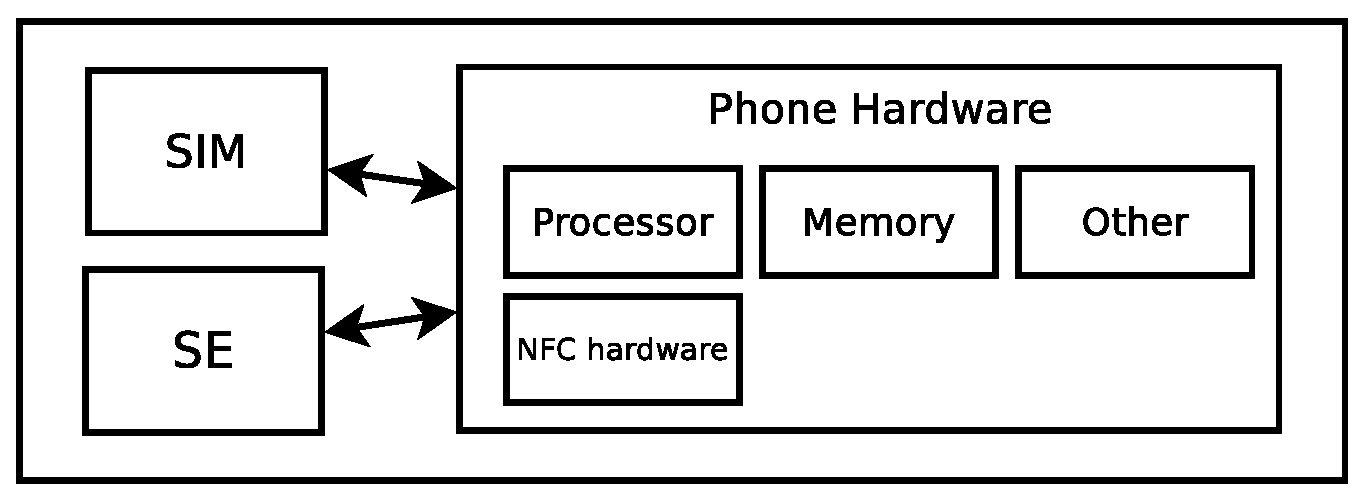
\includegraphics[width=0.5\textwidth]{images/phone_with_SE_nokia}
\caption[Nokia phone with SE]
{
A separate secure element
}
\label{fig:integrated_se}
\end{figure}

\begin{figure}
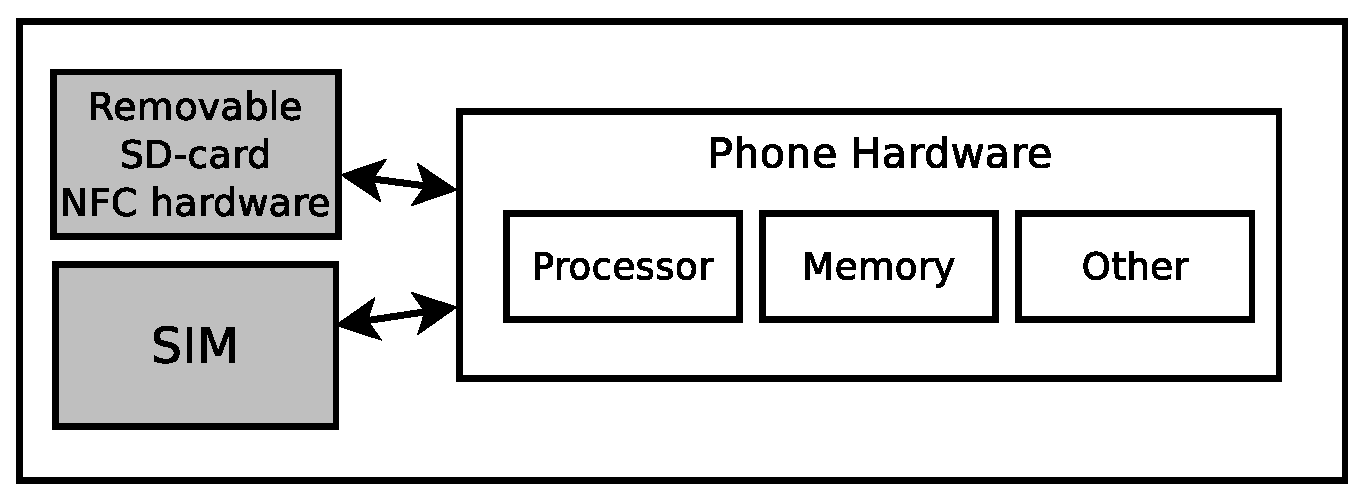
\includegraphics[width=0.5\textwidth]{images/SD_NFC}
\caption[SE in SD package]
{
An secure element in SD package
}
\label{fig:modular_se}
\end{figure}

\begin{figure}
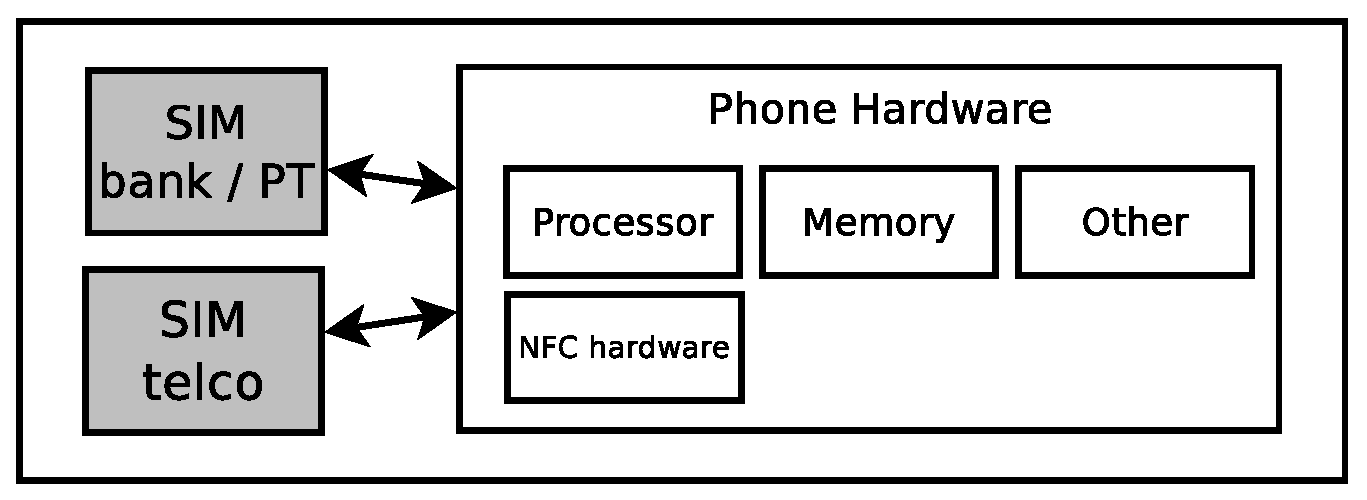
\includegraphics[width=0.5\textwidth]{images/meerdere_sims}
\caption[Multiple SIM cards]
{
Multiple SIM cards for different applications
}
\label{fig:multi_sim}
\end{figure}

\begin{figure}
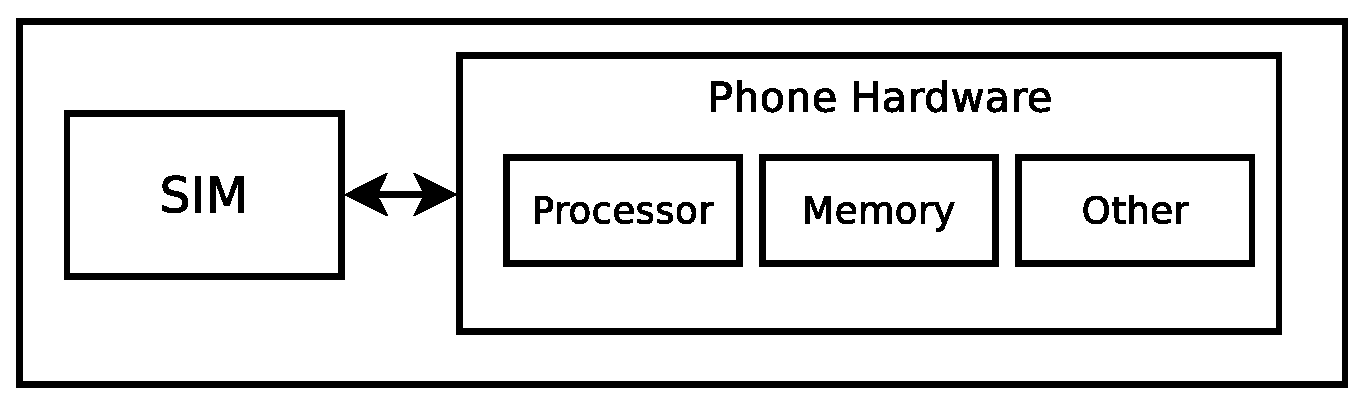
\includegraphics[width=0.5\textwidth]{images/SIM_is_SE}
\caption[Trusted SIM cards]
{
Trusted SIM card running multiple applications
}
\label{fig:sim_se}
\end{figure}




%\cleardoublepage

%\newpage

\bibliographystyle{alpha}
\bibliography{rdr1}
%\printglossaries

\end{document}

